\chapter{Opis projektnog zadatka}
		
		\textbf{\textit{dio 1. revizije}}\\
		    Cilj projekta je razvijanje aplikacije za šahovski klub. Aplikacijom će
			se moći služiti:
			
			\begin{description}
				\item[$\bullet$] treneri 
				\item[$\bullet$] članovi
				\item[$\bullet$] neregistrirani korisnici
			\end{description} 
		    Aplikacijom će upravljati administrator. Jedna osoba može imati samo jednu od ove
			četiri uloge. Glavne koristi aplikacije su interaktivno učenje šaha,
			natjecanje protiv drugih članova kluba u turnirima i infomiranje članova
			o aktivnostima i novostima u klubu. Članovi mogu preko aplikacije plaćati članarinu. Korisnici će učiti šah pomoću dnevnih šahovskih
			taktika, koje postavljaju treneri. Treneri mogu organizirati turnire,
			organizirati treninge i informirati članove pomoću stranice s novostima.
			Neregistrirani korisnici imat će ograničene mogućnosti kod korištenja
			aplikacije. \\
		    Korisnik koji prvi puta pokreće aplikaciju i nije registriran smjeti će
			pristupiti novostima i informirati se o svim događanjima u klubu,
			rješavati dnevne šahovske taktike, ali neće biti dio rang lista, na
			kojima će biti popisani najuspješniji članovi koji su rješavali dnevne
			taktike. Status člana potreban je i za pristup organiziranim treninzima
			i turnirima. Ukoliko je korisnik zainteresiran za učlanjenje u klub,
			smjeti će napraviti korisnički račun, za koji su potrebni:
			\begin{description}
			\item[$\bullet$] korisničko ime
			\item[$\bullet$] e-mail
			\item[$\bullet$] lozinka. 
	    	\end{description} 
			Pri izradi računa korisnik se mora složiti s
			pravilima kluba (ne smije varati pomoću \textit{``chess engine''}-a , ne smije
			koristiti tuđi korisnički račun ili dati svoj drugima na korištenje, ne
			smije se neprikladno ponašati prema trenerima ili drugim članovima...).
			Nakon uspješne registracije, kako bi dobio status člana, registrirani
			korisnik mora platiti članarinu. Nakon ispunjavanja formulara u koji se
			upisuju ime i prezime člana, mjesec za koji se članarina plaća, dob,
			broj mobitela i e-mail adresa, ako je transakcija uspješno provedena
			administrator korisniku dodjeljuje status člana. Status člana bit će
			maknut ukoliko korisnik prestane plaćati članarinu, tj. transakcija za
			određeni mjesec ne bude provedena i upisana u bazu podataka. Članovi uz
			rješavanje taktike imaju mogućnost dodijeliti ocjenu taktici ovisno o
			njenoj težini (1-5), a u slučaju da misle da postoji pogreška u taktici
			ili vide bolje rješenje, mogu prijaviti pogrešku. Rang liste za taktike
			rade se ovisno o vremenu koje je članu potrebno da točno riješi taktiku
			i težini taktike. U aplikaciji postoje rang liste koje prikazuju
			najbolje rješavače taktika. Nove rang liste postavljaju se svaki mjesec.
			U taktici je dozvoljen samo jedan poredak poteza, a u slučaju pogrešnog
			poteza rješavaču se dodaje vremenska kazna (1 minuta) za svaki pogrešan
			potez. Ako član misli da je uočio pogrešku u taktici, može je prijaviti
			tako da nakon pritiska na gumb za prijavu pogreške u otvorenu simulaciju
			taktike unese poteze za koje misli da su ispravni i dodatno obrazloži
			poteze u tekstualnoj kućici ako smatra da je potrebno. Ako član želi
			dodatno vježbati, može se prijaviti na organizirani trening kod trenera.
			Trener u opisu treninga navodi što će sve biti uključeno u njegov
			trening. Nakon vježbanja član može testirati svoju vještinu protiv
			drugih igrača u sklopu turnira. Na stranici turnira član može vidjeti
			raspored nadolazećih turnira i prijaviti se ako ima slobodnih mjesta.
			Turniri se održavaju u točno određeno vrijeme. Tada članovi koji su se
			prijavili igraju jedan protiv drugog sve dok se ne proglasi pobjednik
			(igre se ne odvijaju u sklopu aplikacije). Turniri se održavaju u
			različitim formatima:
			\begin{description} 
			\item[$\bullet$] \textit{rapid} (25 minuta po igraču)
		    \item[$\bullet$] \textit{blitz} (5 minuta po igraču)
			\item[$\bullet$] \textit{bullet} (2 minute po igraču)
		    \end{description}
			 Na stranici turnira postavlja se
			očekivano ukupno vrijeme trajanja turnira. Treneri uz mogućnost
			organiziranja treninga i turnira mogu postavljati dnevne taktike ili
			objavljivati zanimljivosti i novosti. Ako član prijavi pogrešku u
			taktici, da bi došlo do promjene taktike, trener ju mora odobriti. Ako
			trener misli da je žalba valjana, on mijenja taktiku i automatski se
			oduzimaju bodovi za članove koji su riješili pogrešnu verziju taktike,
			te se omogućava ponovno rješavanje ispravljene taktike. Najveće ovlasti
			na stranici ima administrator. On smije dodavati bilo kakav sadržaj,
			brisati sadržaj iz svih rubrika i zabraniti pristup bilo kojem članu i
			treneru. Prilikom brisanja sadržaja, on ostaje u bazi podataka, ali se
			ne prikazuje u aplikaciji. Administrator jedini može dodijeliti uloge
			drugim korisnicima. \\
			Postoje aplikacije sa sličnim mogućnostima poput \textit{chess.com} ili \textit{lichess.org}. Tamo
			je moguće napraviti korisnički račun i vježbati na šahovskim taktikama
			na sličan način kao u našoj aplikaciji, ali te stranice nisu toliko
			fokusirane na rad kluba, nego na učenje i igranje šaha. Ovakve stranice
			pružaju razne mogućnosti poput igre jedan na jedan, učenja šahovskih
			otvaranja, igranja protiv \textit{„chess engine``}-a, što naša aplikacija neće
			sadržavati. Naša aplikacija fokusira se na jedan šahovski klub i njegovu
			organizaciju. \\
			
				\begin{figure}[H]
				\centering
				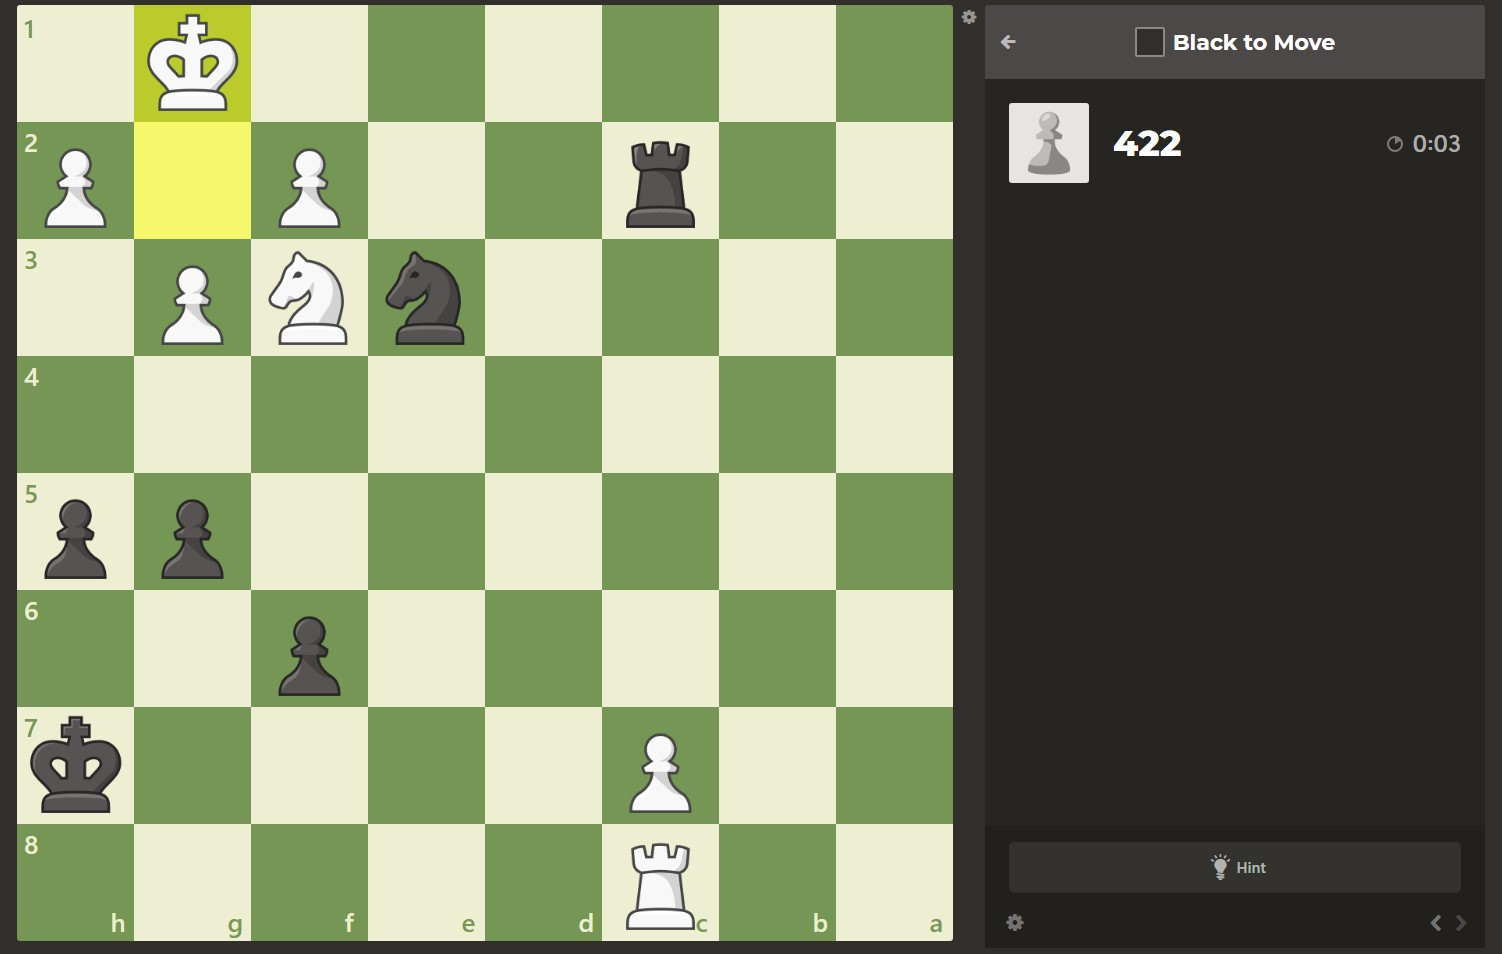
\includegraphics[scale=0.3]{slike/sah-slicno rjesenje.jpeg} %veličina slike u odnosu na originalnu datoteku i pozicija slike
				\caption{Šahovska ploča preuzeta s druge stranice kao primjer drugačijeg rješenja}
				\label{fig:UC$<$broj obrasca$>$}
			\end{figure}
		
	     	\noindent   Za ovakvu aplikaciju mogli bi biti zainteresirani vlasnici šahovskog
			kluba koji žele svojim članovima pružiti više mogućnosti učenja šaha i
			lakši način praćenja novosti u klubu. Postojanje ovakve aplikacije je i
			u interesu svim šahistima koji žele interaktivnije načine sudjelovanja u
			klupskim aktivnostima. Vrlo je vjerojatno da bi šahisti odabrali klub
			koji pruža i online usluge umjesto kluba koji djeluje isključivo uživo. \\
		    Uz sve koristi koje aplikacija pruža, bitno je spomenuti i dosege.
			Projekt omogućava korištenje šahovske ploče za rješavanje dnevnih
			taktika, ali se ne omogućava online igra protiv drugih igrača. Dio
			aplikacije koji se bavi turnirima također ne omogućava 1 na 1 igranje,
			nego samo bilježi raspored turnira i omogućava članovima da se prijave
			na turnir. Organizirani treninzi ne omogućavaju treneru da direktno
			pomoću aplikacije igračima na ploči prikazuje lekcije, nego
			funkcioniraju poput rasporeda gdje članovi mogu vidjeti kada će se
			treninzi održati i kako će izgledati. Dnevne taktike ne omogućavaju
			igračima slobodno postavljanje figurica, nego se koncentriraju na točno
			određenu konfiguraciju ploče. Rješenja dnevnih taktika provjeravaju se
			protiv zadanog slijeda poteza, a ne \textit{``chess engine''}-a (zbog toga se i
			omogućava prijava pogreške u taktici). Prijava pogreške ne sadrži
			dvosmjernu komunikaciju između člana koji se žali i trenera, nego se
			sastoji isključivo od žalbe i mogućeg odobrenja promjene. Aplikacija
			također ne omogućava dvosmjernu komunikaciju (chat) između članova ili
			trenera.\\
			Moguće je nadograditi i proširiti razne aspekte naše aplikacije. Uz
			učenje na dnevnim taktikama moguće je dodati i analiziranje odigranih
			igara ili učenje šahovskih otvaranja. Aplikaciji je moguće dodati neki
			oblik komunikacije između korisnika (forum ili chat). Turniri bi se
			mogli održavati putem aplikacije ako se uz organizacijski aspekt doda i
			mogućnost igranja i bilježenja ratinga, koji bi se računao prema
			uspjehu u igranju protiv drugih članova kluba, a ne samo po uspjehu u
			šahovskim taktikama. Aplikacija bi mogla bilježiti statistike korisnika i
			prikazivati ih na njihovoj osobnoj stranici. Stranici s obavijestima bi
			bilo koristno dodati mogućnost komentiranja na objave. Ukoliko se
			aplikacija želi značajnije proširiti, mogla bi obuhvaćati više šahovskih
			klubova.\\
		    Potencijal za nadogradnju ovog programa u budućnosti svakako bi trebao sadržavati mogućnost testiranja budućih članova i njihovo kategoriziranje u budućem članstvu kluba. To znači da bi budući član osim uplate članarine, koja bi mu omogućila ulaz i korištenje aplikacija šahovskog kluba, trebao proći kroz testne šahovske zadatke koji bi ga prema stupnju uspješnosti stavile u A, B ili C grupu. Primarno grupe ne bi „razbijale“ homogenost šahovskog kluba već bi svakom pojedincu ukazale na stupanj njegovog trenutnog znanja i omogućile kroz treninge i takmičenja njegov rast i napredak. Time bi se statistički moglo pratiti svaki pojedinac. Grupe bi bile određena interna kategorija članova unutar kluba. Samim članovima bio bi izazov pratiti svoju uzlaznu krivulju. \\
		Osim redovne mjesečne članarine trebalo bi omogućiti, kao jednu od budućih nadogradnji kod uplate, opciju da članovi uplaćuju unaprijed za 6 ili 12 mjeseci. Time bi se osim određenih financijskih sredstava koje se korisno mogu utrošiti za razvoj kluba (materijalni i intelektualni troškovi), dobila i jedna stabilna baza igrača na kojoj bi se mogao temeljiti razvoj, ali i opstojnost kluba. Sigurno članstvo osigurava budućnost kluba. Takvim članovima koji se odluče na dugoročnije uplate članarine treba osigurati popuste kod uplate, osigurati određeni reklamni materijal s logom kluba, omogućiti više drugih aktivnosti u samom programu.\\
	    Za pomoć pogledati reference navedene u poglavlju ''Popis literatur'', a po potrebi konzultirati sadržaj na internetu koji nudi dobre smjernice u tom pogledu.
		
		\section{Motivacija za projekt}
		Ideja ovog je projekta olakšati šahovskom klubu obavljanje administrativnih poslova i komunikaciju s članovima. To bi se postiglo web aplikacijom sa funkcionalnostima kao što su online uplaćivanje članarine, objavljivanje novosti, te prijavljivanje članova za treninge i turnire. Web aplikacija bila bi intuitivna i jednostavna za korištenje kako članovima, tako i zaposlenicima kluba. Osim toga, članovi bi se putem web aplikacije mogli nadmetati u rješavanju dnevnih taktika, te tako sudjelovati u šahovskoj zajednici čak i van fizičkog prostora kluba.  \\
Još jedan bitan aspekt ove aplikacije bio bi njen potencijal za nadogradnju. Jasno je da će u budućnosti potrebe šahovskog kluba rasti i da će se trebati uvesti nove funkcionalnosti u web aplikaciju. Tu činjenicu mora odražavati kvaliteta programskog rješenja i dokumentacije kako bi se pružio dobar temelj za nova proširenja.
		
		\eject

		
	